\documentclass[11pt]{article}
\usepackage{cite}
\usepackage{lmodern}
\usepackage[utf8]{inputenc}
\usepackage[finnish]{babel}
\usepackage{hyperref}
\usepackage{graphicx}
\usepackage[figurename=Fig.]{caption}
\usepackage{subfig}


\title{Network Analysis - Project Report}
\author{
    Jimi Hytönen\\
    \and Hanna Holtdirk\\
    \and Basil Mashal
}
\begin{document}

\maketitle

\section{Introduction}
This project is part of network analysis course. The purpose of this project was to analyse a real-world network by applying different algorithms to extract some interesting information about the network as well as get hands-on experience with network analysis. We chose to analyse California road networks, because apart from the roads and nodes there was also additional information available in the form of points of interest, which led to many analysing opportunities.


In this report we will cover the technical aspects of gathering the data, tell how the work was divided, explain our network analysis and visualizations, and finally describe our conclusions. The project can be found in github (https://github.com/Jimmeeee/NA-project).



\section{Data}

We used dataset from https://www.cs.utah.edu/~lifeifei/SpatialDataset.html which was collected, cleaned and formatted from multiple different sources into easy-to-use format. Network's nodes were in longitude-latitude coordinate form and network's edges contained information about start node, end node and the distance between them. In addition, the site provided information about California's points of interest such as hospitals, lakes and airports. There was also an additional map format, which contained the edges with length and the points of interest on the edge. 

We used pandas for data manipulation and processing as we needed to get the data into a certain form for further analysis. We used networkx for building and visualization of the network. This was really straightforward to do as the data was in an easy to use format.  

\newpage

\section{Methods}
For the project we divided the original question into the following subtasks: 
\begin{enumerate}
\item What is the general structure of the road network?
\item Can we find where the (big) cities are from the road network and points of interest?
\item Can we learn to make predictions about the placement of the roads and places of interest?
\end{enumerate}

For each of these subtasks we planned what analysis was needed to answer the question. After setting these subtasks we created a timeline for the project. 
\\
For the first question we analyzed the California road network with simple methods to get a better idea what we are dealing with. One of which was calculating the connectivity of the network to determine if there were roads that led nowhere. Another one was calculating the clustering coefficient to determine the tightness of the network. We also calculated and visualized different centrality measures of the network such as degree centrality, betweenness centrality, eigenvector centrality and katz centrality. 
\\
After analyzing the general structure of the network, we moved to the second question. For finding the big cities we used Girvan Newman community detection algorithm as it seemed to be the most suitable for the task. However, we didn't use the standard method for determining the edge to remove in each iteration, because this would take far too long on our big network, which we already noticed in part one when we calculated the betweenness centrality. Therefore, we used an approximation of the betweenness centrality (only considering 20 nodes each time) and also took the number of points of interest on an edge into account.
\\
For the third question, we did a link prediction for the roads and a classification for the points of interest. We only did these on one of the calculated communities because of the size of the network. 
First, we formulated the road prediction as a classification task by defining class 0 as node pairs with no edge and class 1 as node pairs with an edge. We then separated all possible node pairs into a training and a test set, where each node pair was represented by a feature vector. We used quadratic discriminant analysis because we where familiar with this method and it seemed to work well (see later for evaluation). Using that, we fit the training data to the model and predicted the classes of the test data. Subsequently, we evaluated the prediction by calculating the number of misclassifications and gaining an accuracy. 
For the classification of points of interest we chose the category as the class. Because there are very many different categories, we chose to only use lake, airport and church. Between these we seemed to be able to classify pretty well (see results). The rest worked similar to the link prediction. 
\\
\section{Results}
\subsection{General structure analysis results}

\subsubsection{Visualization}
From the visualization of the network, we can see that it only depicts the bigger roads and that there seem to be nodes strewn across the big roads to determine the exact course of the road. Furthermore with the additional points of interest, we can already see where the big cities seem to be located. 
\begin{figure}[h!]
    \centering
    \caption{California's road network}%
    \subfloat[Edges of the network]{{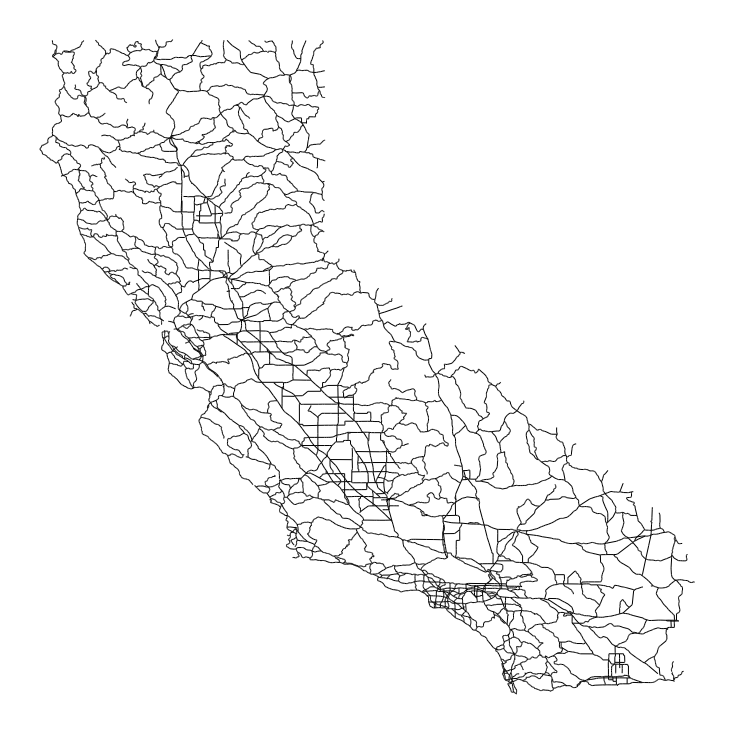
\includegraphics[width=5.5cm]{road.png} }}%
    \qquad
    \subfloat[Points of interest]{{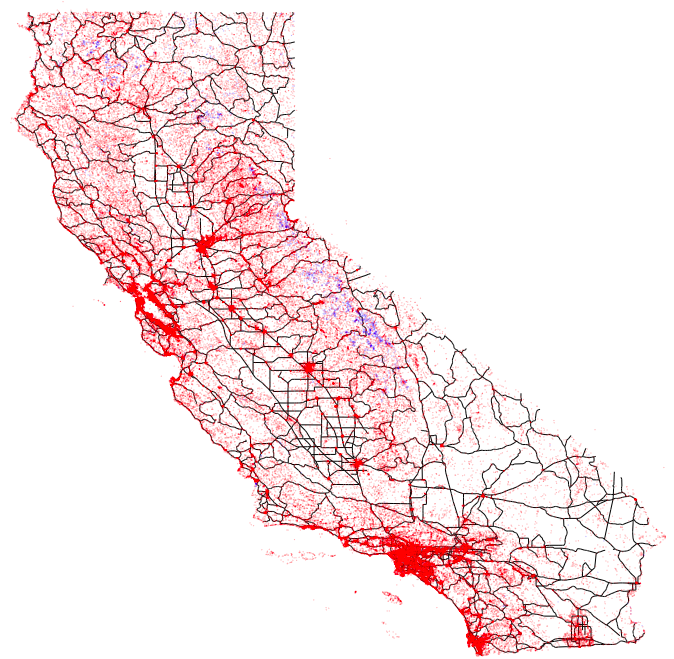
\includegraphics[width=5.5cm]{pois.png} }}%
\end{figure}


\subsubsection{Connectivity, Degree Distribution and Clustering Coefficient}
We found out that California's roads are connected and there are no isolated sections, which is to be expected. Furthermore, from Figure \ref{fig:degree}, we can see the node degree distribution. As implied in 4.1.1, the majority of the nodes have degree of two as they are the middle nodes of the road. However, we can also see that there are some nodes that have degree higher than two. They are the intersections, where a three-way junction is most common followed by a four-ways and only a few bigger ones. There are also 182 dead-ends (nodes with degree of one).
The average global clustering coefficient is ca. 0.000071 with 21042 nodes having a value of 0 and only 3 nodes with a coefficient of 0.17 or 0.33 respectively. This means that for most nodes the neighbours are not connected, which makes sense given the above discovery. 

\begin{figure}[h]
\caption{Degree distribution}
\label{fig:degree}
\centering
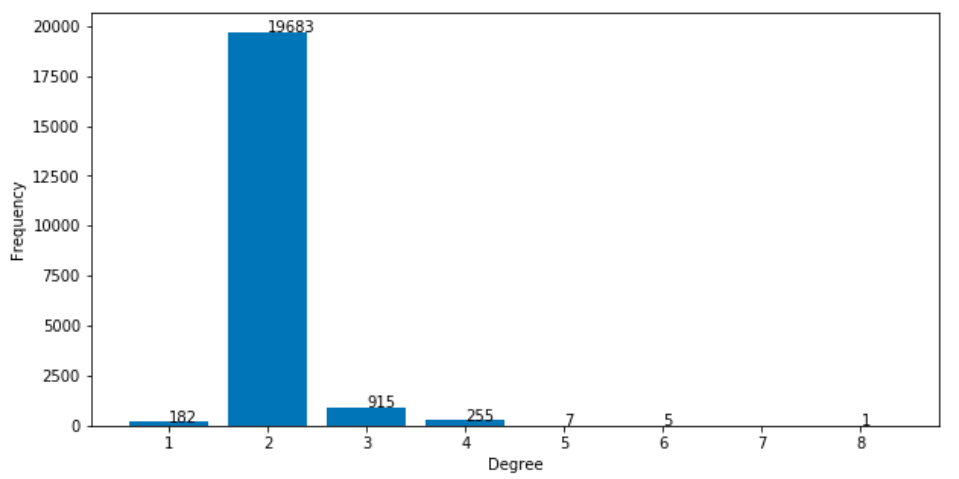
\includegraphics[scale=0.3]{degree.png}
\end{figure}

\subsubsection{Centrality}
In Figure \ref{fig:centrality}, we can see the different centrality measures, where higher color intensity and bigger node size means higher centrality value.  We can see that the betweenness centrality contains the most valuable information of the network because it indicates where the important roads lie. They seem to go from north to south, parallel to the coast line.

\begin{figure}[h]
\centering
    \caption{Centrality measures}%
    \label{fig:centrality}
    \subfloat[Degree centrality]{{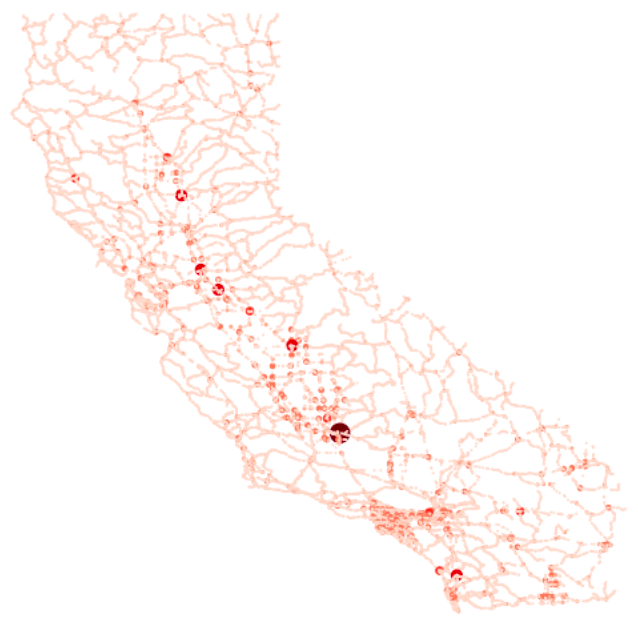
\includegraphics[width=4.5cm]{centrality_deg.png} }}%
    \qquad
    \subfloat[Betweenness centrality]{{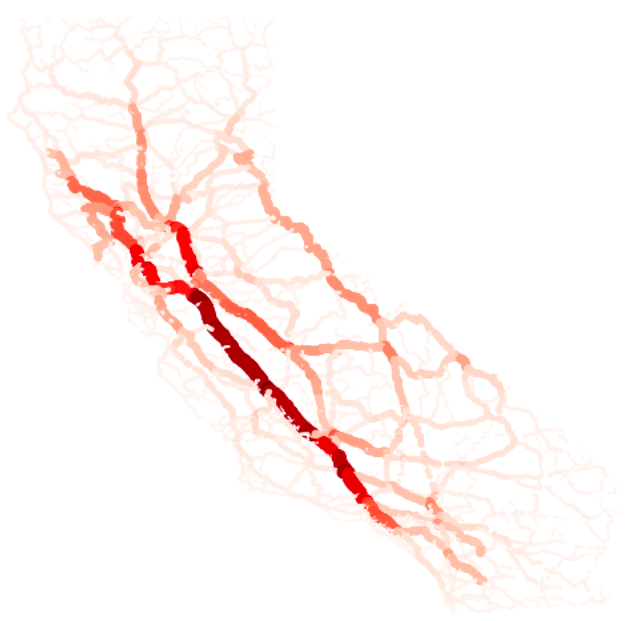
\includegraphics[width=4.5cm]{centrality_betw.png} }}%
    \qquad
    \subfloat[Eigenvector centrality]{{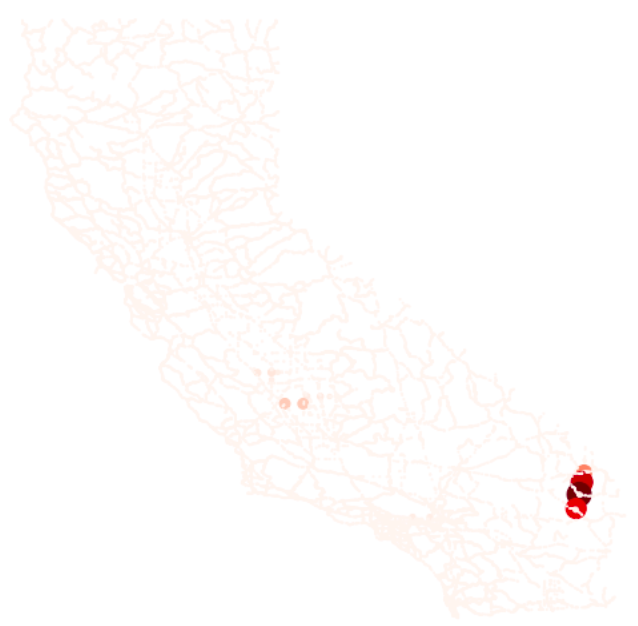
\includegraphics[width=4.5cm]{centrality_eig.png} }}%
    \qquad
    \subfloat[Katz centrality]{{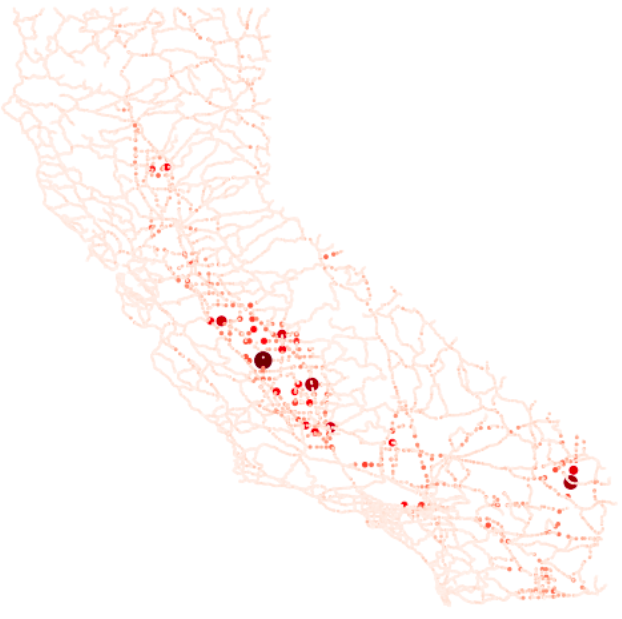
\includegraphics[width=4.5cm]{centrality_katz.png} }}%
    
    \caption{Girvan Newman community detection}
\label{fig:com}
\centering
 \subfloat[Communities]{{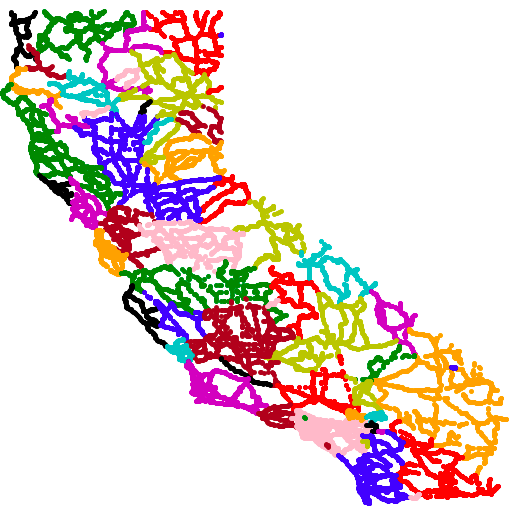
\includegraphics[width=6cm]{communities.png} }}%
 \qquad
 \subfloat[Counties of California]{{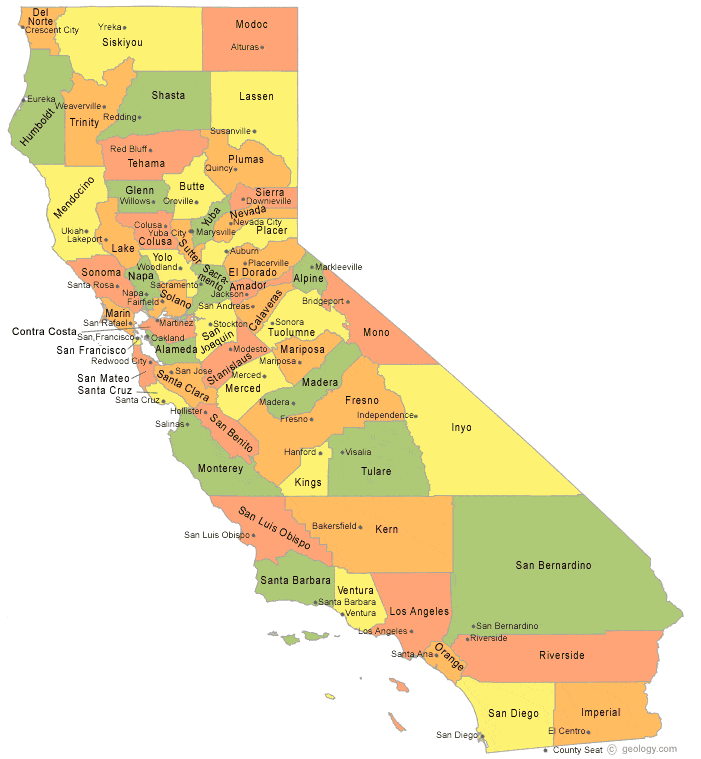
\includegraphics[width=5.5cm]{counties.png} }}%
\end{figure}


\subsection{Communitites}
At first, we wanted to find the cities through the community detection, but we discovered that we can better detect the counties of California. Therefore, we ran our own version of the Girvan Newman algorithm (see methods) until we have 58 communities as there are 58 counties. 
In Figure \ref{fig:com}, we can see how well we managed to find different counties based on the road network. 

\newpage
\subsection{Predictions through Machine Learning}
The road prediction works really well for the network. We have an average accuracy of 99\%. We tried different features and discovered that distance between the nodes and number of points of interest (of type airport) between the nodes (with some variance) seem to bring the best results, where the first feature is the most deciding one. We discovered this by leaving one feature out and comparing the false positives and false negatives (if we only compare the accuracies this may be misleading because there are far fewer node pairs of class 1 than 0 and always printing 0 would give a good accuracy). \\
The classification of the points of interest was a little bit harder, but we now have an average accuracy of 85\% when classifying between lake, airport and church. The chosen features are: amount of other pois in a close distance, distance to nearest poi of the same class, distance to nearest road node and position. What feature is most deciding varies based on the community that is being analyzed. \\
Originally we also wanted to learn what buildings there should be in a community and where they should be placed. Because of time limitations and the amount of categories, we decided against doing this task. 

\section{Conclusion}
The aim of the project was to analyze the structure and communities of the road network and points of interest of California and try to make predictions about them. For this we used methods like degree distribution, centrality measures, community detection, link prediction and node classification.
The results show that the data seems to be made for visualization. The only node attributes are the position and only the big roads are depicted using many intermediate nodes to show the course of the roads rather than simply the connections. Furthermore, the Girvan Newman communities seem to correspond to the counties of California. Finally, we were able to make good predictions for the network, which means that the placement of road and points of interest follow a certain structure that can be best described by the features mentioned in the section above.

\end{document}
